\documentclass[12pt]{amsart}
\usepackage{fullpage}
\usepackage{pbox}
\usepackage{graphicx}
\usepackage{booktabs} % Top and bottom rules for table
\usepackage{amsfonts, amsmath, amsthm, amssymb}
\usepackage{longtable,array,color,xcolor}
\usepackage[colorlinks = true,
            urlcolor  = blue]{hyperref}
\usepackage{verbatim}
\usepackage{enumerate}
\newcommand\narrowstyle{\SetTracking{encoding=*}{-50}\lsstyle}

\setlength{\parindent}{0pt}

\begin{document}

\title{Math 320: Homework 1 Solutions}
\maketitle

\begin{enumerate}
\item The following code defines a function {\tt rho} which inputs
the temperature and outputs the density. We use {\tt arrayfun}
to apply it to a range of temperatures. Then we plot the result.

\begin{verbatim}
rho = (@(TC) 5.5289e-8 * TC^3 - 8.5016e-6 * TC^2 + 6.5622e-5*TC + .99987)
tempsF = 32:3.6:93.2;               %define the temperature vector
tempsC = (5/9)*(tempsF - 32);       %convert to Celsius.
densities = arrayfun(@(t) rho(t), tempsC);
plot(tempsC,densities)
\end{verbatim}

\begin{figure}[h!]
\centering
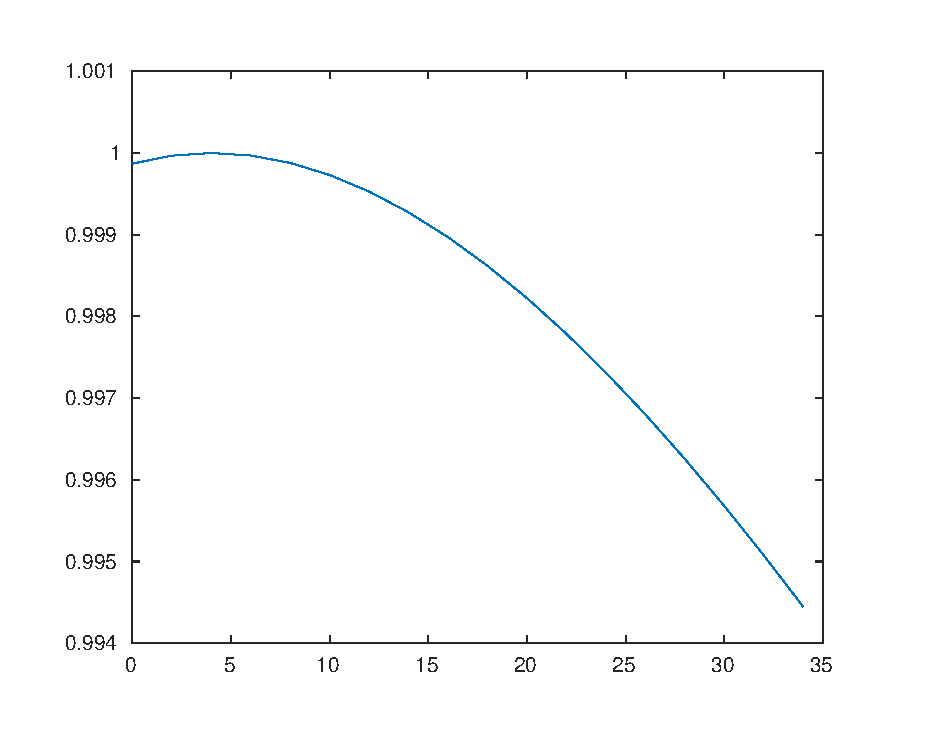
\includegraphics[scale=1]{hw1p1.eps}
\end{figure}

\item First we define the $x$-range $X$. Then we compute both
the cosine function, and the approximation as functions of the array $X$.
Then we plot both together. The option '--' means the second plot
will be a dashed line, while 'k' means it will be black.

\pagebreak

\begin{verbatim}
X = 0:pi/100:3*pi/2;
Y1 = cos(X);
Y2 = 1 - X.^2/factorial(2) + X.^4/factorial(4) ...
    - X.^6/factorial(6) + X.^8/factorial(8);
plot(X,Y1,X,Y2,'--k')
\end{verbatim}

\begin{figure}[h!]
\centering
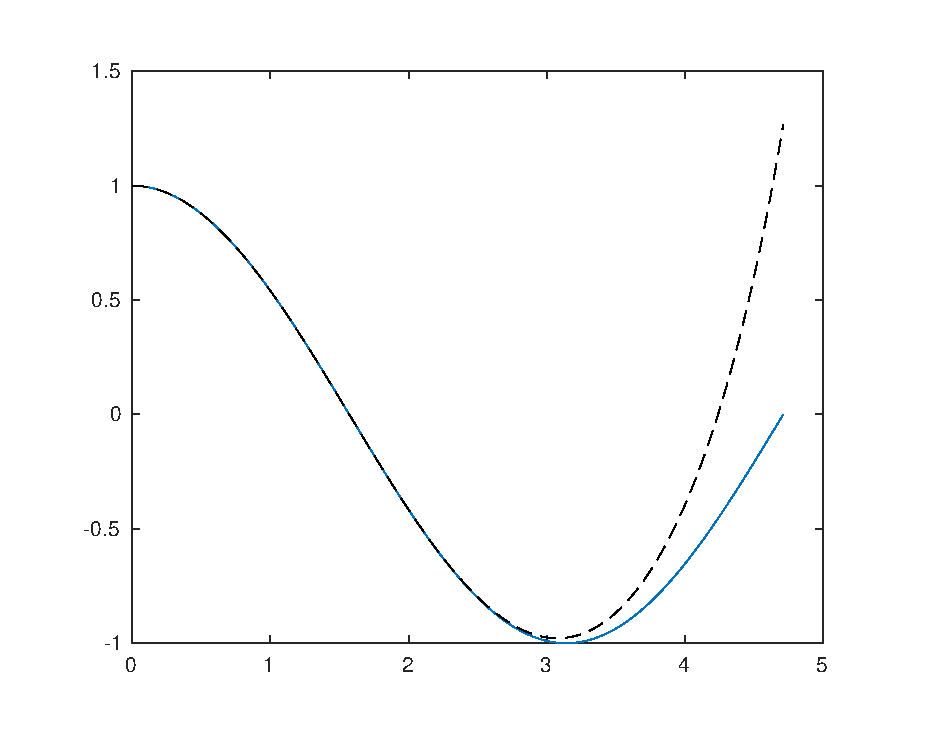
\includegraphics[scale=1]{hw1p2.eps}
\end{figure}

\vspace{1cm}

\item First we set up the MATLAB function
PolarForm with all {\tt if ... elseif} cases.
$r$ can be evaluated first, since the formula is
always the same. Note that some {\tt if} statements are
nested.

\begin{verbatim}
function polar = polarForm(x,y)
%input: x,y coming from z =  x + i*y
%ouptut: r, theta for which re^(i*theta) = z
%r has the same formula everywhere, theta has
%different values for different cases.
r = sqrt(x^2 + y^2);
if x > 0
    theta = atan(y/x);
elseif x < 0
    if y > 0
        theta = atan(y/x) + pi;
    elseif y == 0
        theta = pi;
    elseif y < 0
        theta = atan(y/x) - pi;
    end
elseif x == 0
    if y > 0
        theta = pi/2;
    elseif y == 0
        theta = 0;
    elseif y < 0
        theta = -pi/2;
    end
end
polar = [r, theta];
end

\end{verbatim}

Then, in order to execute the code, we use
the following code which reads in each point,
and then adds the $(r,\theta)$ value as a new
column in a matrix $L$. The final command
simply prints the values to the screen.


\begin{verbatim}
X = [2,2,0,-3,-2,-1,0,0,2];
Y = [0,1,3,1,0,-2,0,-2,2];

L = zeros(9,4);
for i=1:9
    L(i,1:2) = [X(i),Y(i)];
    v  = polarForm(X(i),Y(i));
    L(i,3:4) = [v(1),v(2)];
end
L
\end{verbatim}

The output is:
\begin{small}
\begin{verbatim}
L =
   2.000000000000000                   0   2.000000000000000                   0
   2.000000000000000   1.000000000000000   2.236067977499790   0.463647609000806
                   0   3.000000000000000   3.000000000000000   1.570796326794897
  -3.000000000000000   1.000000000000000   3.162277660168380   2.819842099193151
  -2.000000000000000                   0   2.000000000000000   3.141592653589793
  -1.000000000000000  -2.000000000000000   2.236067977499790  -2.034443935795703
                   0                   0                   0                   0
                   0  -2.000000000000000   2.000000000000000  -1.570796326794897
   2.000000000000000   2.000000000000000   2.828427124746190   0.785398163397448
\end{verbatim}
\end{small}
\vspace{1cm}

\item The first thing is to define a function that outputs
the desired quantities. We call this function {\tt dotCross}.
Note that I use a subfunction {\tt mgd} to return the magnitude
of a vector. I also used a subfunction {\tt crossP} which uses
the standard determinant definition, but the built-in function
{\tt cross} is perfectly acceptable.

In order to plot the three vectors, we use plot3 on a set of
two points: the origin, and the vector coordinates. 
We add in the option '--' so that the first two lines are dashed.
\begin{verbatim}
function [theta,c,mag] = dotCross(a,b)
%Input: two vectors in R^3
%Output: the angle between them, the cross
%product, and the magnitude of the cross product.
theta = acos(sum(a.*b)/(mgd(a)*mgd(b)));
c = crossP(a,b);
mag = mgd(c);
A = [zeros(1,3);a];
B = [zeros(1,3);b];
C = [zeros(1,3);c];
plot3(A(:,1),A(:,2),A(:,3),'--',...
    B(:,1),B(:,2),B(:,3),'--',...
    C(:,1),C(:,2),C(:,3));
end

function x = mgd(v)
%Input: vector
%Output: magnitude of the vector
x = sqrt(sum(v.^2));
end

function w = crossP(a,b)
%Input: pair of vectors
%Output: cross product of vectors.
m = [a;b];
w = [det([m(:,2) m(:,3)]),...
    -det([m(:,1) m(:,3)]),...
    det([m(:,1) m(:,2)])];
end
\end{verbatim}

In order to evaluate each of the examples, we input the following
code. Note that {\tt figure} is called before each call to dotCross
so that the plot is saved in a new figure.

\begin{verbatim}
A = [6 4 2; 3 2 -6; 2 -2 1; -1 0 0];
B = [2 6 4; 4 -3 1; 4 2 -4; 0 -1 0];

thetaList = zeros(1,4);
cList = zeros(4,3);
magList = zeros(1,4);
for i = 1:4
    figure;
    [theta, c, mag] = dotCross(A(i,:),B(i,:));
    thetaList(i)= theta;
    cList(i,:) = c;
    magList(i) = mag;
end
thetaList
cList
magList
\end{verbatim}

The output revealed is:

\begin{verbatim}
thetaList =

    0.6669    1.5708    1.5708    1.5708

cList =

    4.0000  -20.0000   28.0000
  -16.0000  -27.0000  -17.0000
    6.0000   12.0000   12.0000
         0         0    1.0000

magList =

   34.6410   35.6931   18.0000    1.0000
\end{verbatim}
The cross-product vectors are read from left to
right.

\vfill
\pagebreak

The graphical displays that are plotted by the {\tt dotCross}
function are included below:


\begin{tabular}{cc}
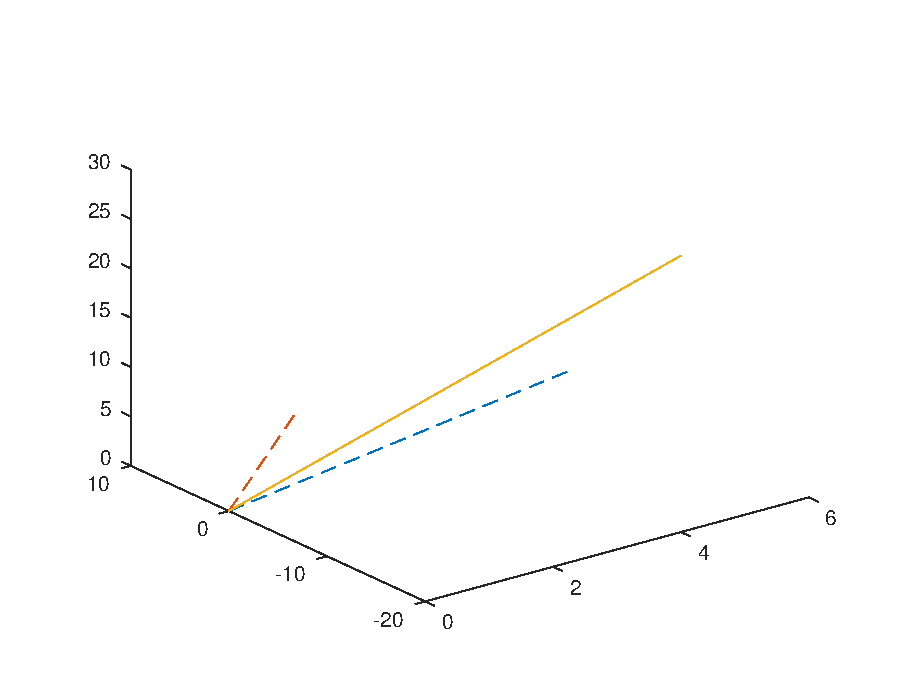
\includegraphics[scale=.5]{hw1p4a.eps} & 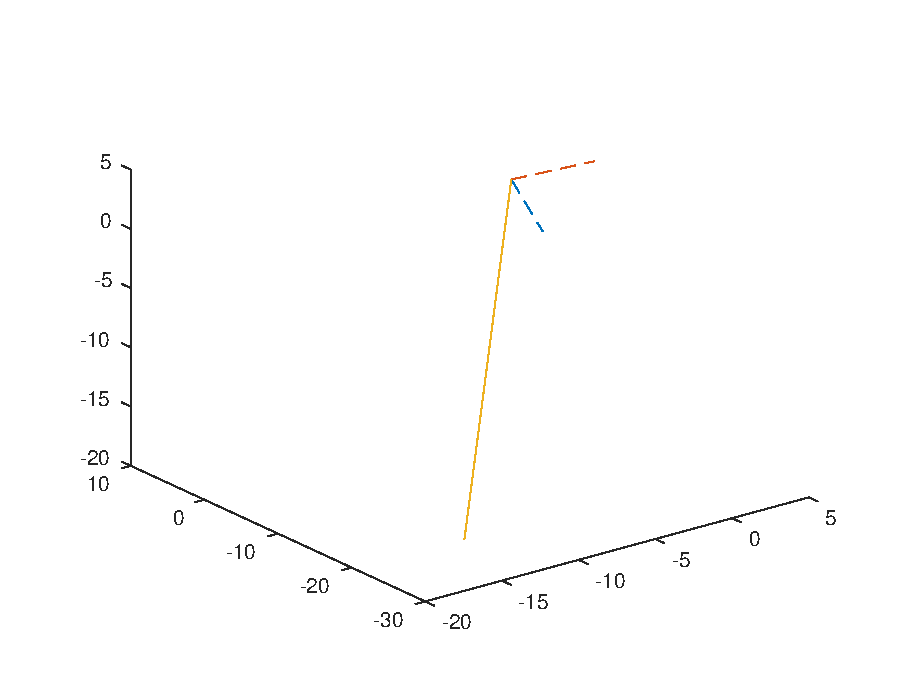
\includegraphics[scale=.5]{hw1p4b.eps} \\
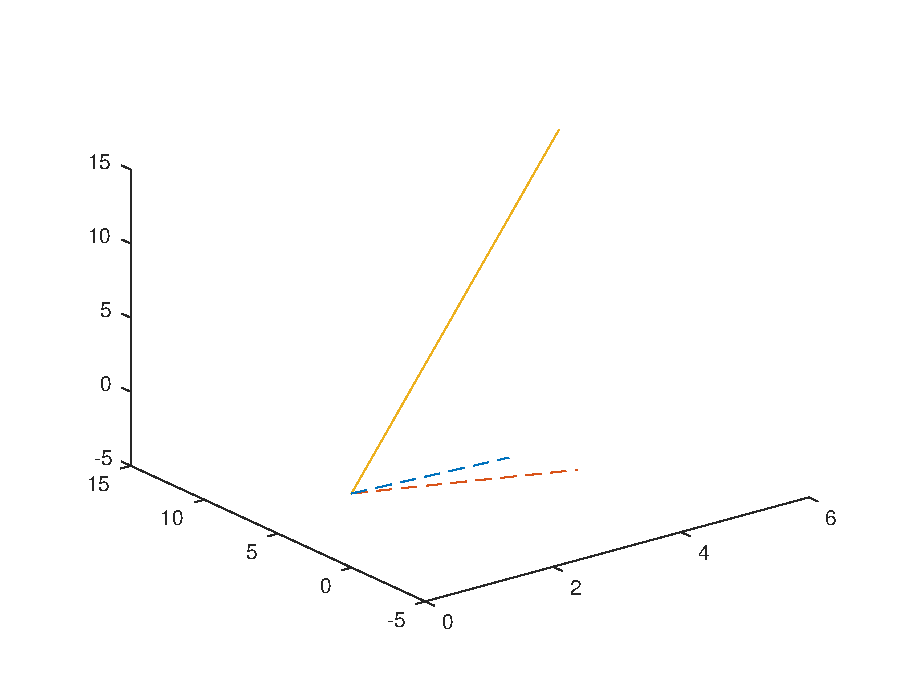
\includegraphics[scale=.5]{hw1p4c.eps} & 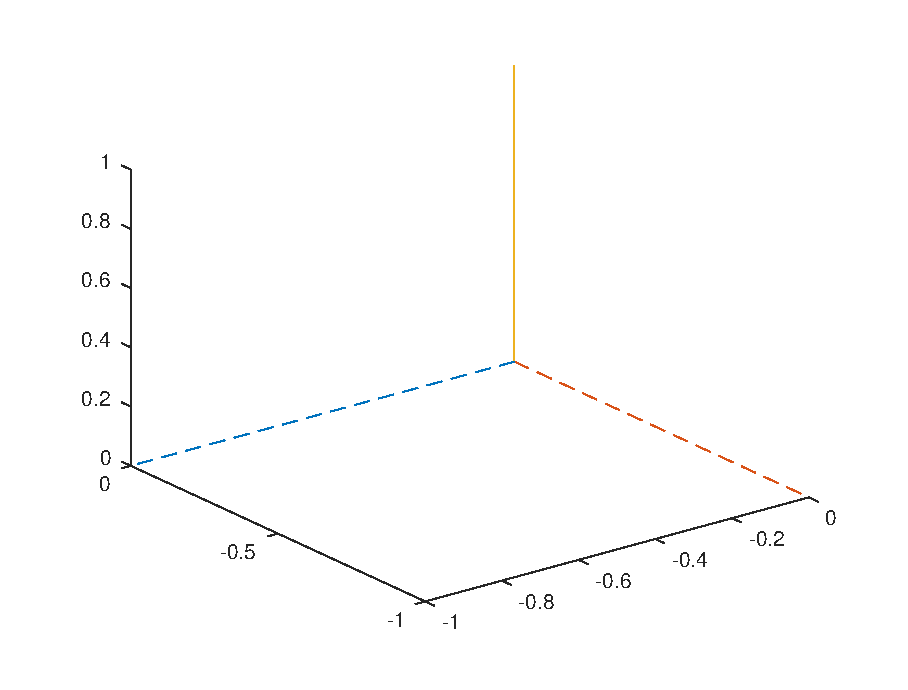
\includegraphics[scale=.5]{hw1p4d.eps} \\
\end{tabular}
\end{document}
